% 95-39(95쪽) — 높이 $15\sqrt{3}\,\mathrm{m}$, $20\sqrt{3}\,\mathrm{m}$ 인 두 건물과 지면의 지점 $\pt{C}$(원문 「오른쪽 그림」). 스캔 화질이 낮아 TikZ 로 다시 그림.
% 라벨은 원문 것만: 두 높이·$60^\circ$ 둘·$\pt{A}$·$\pt{B}$·$\pt{C}$·$\pt{D}$·$\pt{E}$ 와 $\pt{D}$·$\pt{E}$ 의 직각 표시.
% 원문의 건물 삽화는 사각형으로만 옮겼다. $\seg{AB}$ 의 길이(답)가 읽히지 않게 눈금·거리는 적지 않는다.
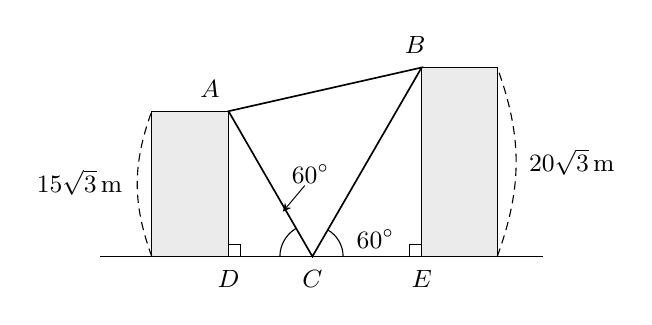
\begin{tikzpicture}[line width=0.6pt, x=0.75cm, y=0.75cm, >=stealth]
  \draw[line width=0.6pt] (-3.6,0) -- (3.9,0);
  \draw[fill=black!8, line width=0.5pt] (-2.72,0) rectangle (-1.42,2.46);
  \draw[fill=black!8, line width=0.5pt] (1.85,0) rectangle (3.13,3.20);
  \draw (-1.42,2.46) -- (0,0) -- (1.85,3.20) -- cycle;
  \draw[line width=0.4pt] (-1.22,0) -- (-1.22,0.2) -- (-1.42,0.2);
  \draw[line width=0.4pt] (1.65,0) -- (1.65,0.2) -- (1.85,0.2);
  \draw[densely dashed, line width=0.4pt] (-2.72,0) to[bend left=20] (-2.72,2.46);
  \draw[densely dashed, line width=0.4pt] (3.13,0) to[bend right=20] (3.13,3.20);
  \node[anchor=east, font=\small] at (-3.05,1.25) {$15\sqrt{3}\,\mathrm{m}$};
  \node[anchor=west, font=\small] at (3.50,1.60) {$20\sqrt{3}\,\mathrm{m}$};
  \draw[line width=0.4pt] (-0.275,0.476) arc (120:180:0.55);
  \node[font=\small] at (-0.03,1.40) {$60^\circ$};
  \draw[->, line width=0.35pt] (-0.13,1.20) -- (-0.50,0.76);
  \draw[line width=0.4pt] (0.52,0) arc (0:60:0.52);
  \node[anchor=west, font=\small] at (0.58,0.30) {$60^\circ$};
  \node[anchor=south east, font=\small] at (-1.40,2.52) {$\pt{A}$};
  \node[anchor=south, font=\small] at (1.74,3.26) {$\pt{B}$};
  \node[anchor=north, font=\small] at (-1.42,-0.06) {$\pt{D}$};
  \node[anchor=north, font=\small] at (0,-0.06) {$\pt{C}$};
  \node[anchor=north, font=\small] at (1.85,-0.06) {$\pt{E}$};
\end{tikzpicture}
